\documentclass[12pt,a4paper]{article}
\usepackage[utf8]{inputenc}
\usepackage[greek,english]{babel}
\usepackage{alphabeta} 
\usepackage[pdftex]{graphicx}
\usepackage[top=1in, bottom=1in, left=0.5in, right=0.5in]{geometry}
\linespread{1}
\setlength{\parskip}{8pt plus2pt minus2pt}
\widowpenalty 10000
\clubpenalty 10000
\newcommand{\eat}[1]{}
\newcommand{\HRule}{\rule{\linewidth}{0.5mm}}
\usepackage[official]{eurosym}
\usepackage{enumitem}
\setlist{nolistsep,noitemsep}
\usepackage[hidelinks]{hyperref}
\usepackage{cite}
\usepackage{lipsum}
\graphicspath{ {./images/} }
\usepackage{listings}
\usepackage{color}
\setlength{\parindent}{0pt}


\definecolor{dkgreen}{rgb}{0,0.6,0}
\definecolor{gray}{rgb}{0.5,0.5,0.5}
\definecolor{mauve}{rgb}{0.58,0,0.82}


\lstset{frame=tb,
	language=C,
	aboveskip=3mm,
	belowskip=3mm,
	showstringspaces=false,
	columns=flexible,
	basicstyle={\small\ttfamily},
	numbers=none,
	numberstyle=\tiny\color{gray},
	keywordstyle=\color{blue},
	commentstyle=\color{dkgreen},
	stringstyle=\color{mauve},
	breaklines=true,
	breakatwhitespace=true,
	tabsize=3
}


\title{ECE 351 Lab 11}
\author{Zachary DeLuca}
\date{April 18th 2023}

\begin{document}
	
\maketitle
\hline
\section*{Introduction}
	In this lab we will be using python to graph the poles of a discrete transfer function. We first need to take the function and find its z transform equivalent. After we transform it, we transform it back into the k domain but altered to be much more manageable.  

\section*{Derivation}

$$y[k] = 2x[k] - 40x[k - 1] + 10y[k - 1] - 16y[k - 2]$$
$$Y(z)=2X(z)-40X(z)z^{-1}+10Y(z)z^{-1}-16Y(z)z^{-2}$$
$$Y(1-10z^{-1}+16z^{-2})=X(2+z^{-1})$$
$$H(z)=\frac{2+z^{-1}}{1-10z^{-1}+16z^{-2}}$$
$$\frac{H(z)}{z}=\frac{2z+1}{z^2-10z+16}=\frac{A}{z-8}+\frac{B}{z-2}=\frac{-4}{z-8}+\frac{6}{z-2}$$
$$h[k]=(-4(8)^k+6(2)^k)u[k]$$


\section*{Graphs}

Using the hand derivations, we can see that this function should have two poles at 2 and 8. When we use the residue function we find we have poles at 2 and 8 using the print function. \vspace*{12pt}

\begin{center}
	{Figure 11.1}
	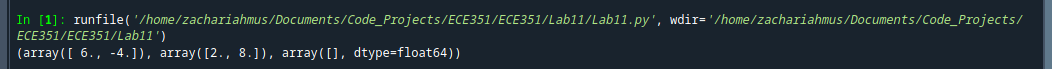
\includegraphics[width = 7in]{/home/zachariahmus/Documents/Code_Projects/ECE351/ECE351/Lab11/2023-04-19_13-28.png}
\end{center}

The next thing to be done is to graph the transform using the provided zplane function and the standard freqz function. 
%$$4(8)^k=6(2)^k$$
%$$\frac{2}{3}8^k=2^k$$
%$$\frac{2}{3}2^{3k}=2^k$$
%$$\frac{3}{2}=2^{2k}$$
%$$ln(\frac{3}{2})=ln(2^{2k})=2kln(2)$$
%$$2k=\frac{ln(2)}{ln(\frac{3}{2})}$$

\begin{center}
	{Figure 11.2}
	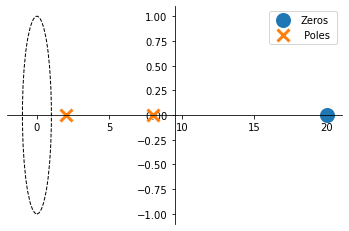
\includegraphics[width = 7in]{/home/zachariahmus/Documents/Code_Projects/ECE351/ECE351/Lab11/Figure 2023-04-19 134615.png}
\end{center}
\vspace{12pt}

\section*{Post Lab Questions}

1. Looking at the plot generated in Task 4, is H(z) stable? Explain why or why not.\vspace{12pt}

The plot shows that the poles exist outside the circle and thus show that the system is not stable. 

\section*{Conclusion}

In this lab we took a look at ta z transformed discrete function and found its zeros and poles. We used these along with some predefined functions to check the stability of the system and we found that the transfer function was unstable for this system. 	

\end{document}
